\documentclass[12pt,twosides,onecolumn,openany]{article}
\usepackage{graphicx} 


\usepackage[catalan]{babel}
\usepackage{emptypage}
\usepackage{hyperref}
\usepackage{mathtools}
\usepackage{blindtext}
\usepackage{subfigure}
\usepackage[utf8]{inputenc}
\usepackage{caption}
\usepackage{subcaption}
\usepackage{wrapfig}
\usepackage[a4paper]{geometry}
\geometry{top=2.5cm, bottom=2.5cm, left=2.5cm, right=2.5cm}
\usepackage{fancyhdr}
\pagestyle{fancy}
\usepackage{amsmath}
\usepackage{amssymb}
\usepackage{amsfonts}
\providecommand{\norm}[1]{\lVert#1\rVert}
\hypersetup{colorlinks=true,urlcolor=blue,linkcolor=blue}
\usepackage{multirow}
\usepackage{multicol}
\usepackage{rotating}

\usepackage{titlesec}

\newenvironment{Figura}
  {\par\medskip\noindent\minipage{\linewidth}}
  {\endminipage\par\medskip}

\titleformat{\section}  % comando de sección a formatear
  {\fontsize{14}{16}\bfseries} % formato para toda la línea
  {\thesection} % cómo mostrar el número
  {0.4em} % espacio entre el número y el texto
  {} % formato solo para el texto
  [] % formato para después del texto


\fancyhf{}
\fancyhead[LO,RE]{Grup D3}
\fancyhead[RO,LE]{Pràctica IIIb}
\fancyfoot[LO,RE]{\thepage}
\fancyfoot[RO,LE]{Laboratori de Termodinàmica - UAB}
\graphicspath{ {images/} }

\begin{document}

\begin{center}
    {\Large \textsc{Gasos reals: Isotermes d'Andrews - Estudi del punt crític}}\\
    \vspace{0.2cm}
    \textsc{3 d'Octubre de 2024}\\
    \vspace{0.2cm}
    Miguel A. - 1637738
\end{center}
\begin{center}
    \textsc{\textit{RESUM}}
\end{center}
Lorem ipsum dolor sit amet, consectetur adipiscing elit, sed do eiusmod tempor incididunt ut labore et dolore magna aliqua. Ut enim ad minim veniam, quis nostrud exercitation ullamco laboris nisi ut aliquip ex ea commodo consequat. Duis aute irure dolor in reprehenderit in voluptate velit esse cillum dolore eu fugiat nulla pariatur. Excepteur sint occaecat cupidatat non proident, sunt in culpa qui officia deserunt mollit anim id est laborum. \cite{prueba}
\vspace{0.5cm}
\begin{multicols}{2}
    \section{Introducció i objecctius}
    Lorem ipsum dolor sit amet, consectetur adipiscing elit, sed do 
    eiusmod tempor incididunt ut labore et dolore magna aliqua. Ut enim ad minim veniam, quis nostrud exercitation ullamco laboris nisi ut aliquip ex ea commodo consequat. Duis aute irure dolor in reprehenderit in voluptate velit esse cillum dolore eu fugiat nulla pariatur. Excepteur sint occaecat cupidatat non proident, sunt in culpa qui officia deserunt mollit anim id est laborum.
    
    \section{Fonament teòric}
    Lorem ipsum dolor sit amet, consectetur adipiscing elit, sed do eiusmod tempor incididunt ut labore et dolore magna aliqua. Ut enim ad minim veniam, quis nostrud exercitation ullamco laboris nisi ut aliquip ex ea commodo consequat. Duis aute irure dolor in reprehenderit in voluptate velit esse cillum dolore eu fugiat nulla pariatur. Excepteur sint occaecat cupidatat non proident, sunt in culpa qui officia deserunt mollit anim id est laborum. \cite{10.1063/1.3037344}
    
    \section{Procediment experimental}
    Estudiarem les propietats de l'hexafluorur de sofre (SF$_6$) en condicions isotèrmiques al voltant del punt crític.
    
    \section{Resultats i discussió}
    \subsection{Diagrama de Clapeyron}
    A partir de les dades experimentals obtingudes al laboratori (veure Annex II a la Secció \ref{sec:Annex_Dades}) construim el diagrama de Clapeyron que s'observa a la Figura \ref{fig:Diagrama_Clapeyron}.
    
    \begin{Figura}
        \centering
        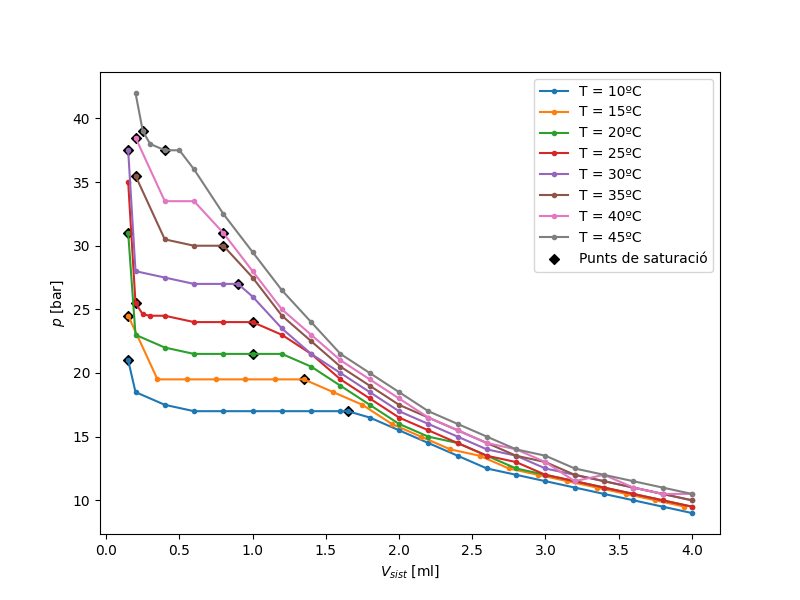
\includegraphics[width=1\linewidth]{../../graphs/practica_IIIb/plots/clapeyron/Clapeyron_v.1.png}
        \captionof{figure}{\footnotesize Diagrama de Clapeyron $p$ vs. $V_{sist}$ per a diferents temperatures.}\label{fig:Diagrama_Clapeyron}
    \end{Figura}

    \section{Conclusions}
    Lorem ipsum dolor sit amet, consectetur adipiscing elit, sed do eiusmod tempor incididunt ut labore et dolore magna aliqua. Ut enim ad minim veniam, quis nostrud exercitation ullamco laboris nisi ut aliquip ex ea commodo consequat. Duis aute irure dolor in reprehenderit in voluptate velit esse cillum dolore eu fugiat nulla pariatur. Excepteur sint occaecat cupidatat non proident, sunt in culpa qui officia deserunt mollit anim id est laborum.
    \section{Annex II: Dades experimentals}\label{sec:Annex_Dades}
\end{multicols}


\end{document}